\begin{enumerate}

\item The rules used to simulate the ant colonies are based on the article Ants 
and the Art of War by M.W. Moffett.  The first of the three rules is:

\begin{myquote}
\textit{An empty cell becomes populated with probability p, majors are 
f $<$ 1 times as likely to be born as minors, and red and blue births are equally 
likely}
\end{myquote}

Allowing red and blue ant births to be equally likely is simply a result of the 
fact that the article mentions a large number of different ant species, each 
forming colonies of similar sizes.  The scarcity of major ants is mentioned 
during the article, when the Moffett states "The medias and majors are much 
scarcer than the minors but far more deadly."

The second rule is:

\begin{myquote}
\textit{A cell of minors becomes empty when surrounded by at least one 
enemy minor or major}
\end{myquote}

The article focuses on the weakness of the smaller "foot soldier" ants, who are 
able to immobilise enemy ants in order for the larget ants to kill them.  The 
article supports the choice to make minors vulnerable to small numbers of other 
minor ants when it is mentioned that 'a single minor has no more chance against 
the children then would an equally small scout of a lone hunting species."

The final rule is:

\begin{myquote}
\textit{A cell of majors becomes empty when surrounded by four minors 
or at least one major}
\end{myquote}

Again, this rule refers to the descriptions of multiple minor ants being needed 
to destroy larger enemy ants.  Moffett also mentions that the major ants are 
'far more lethal', so they would also have an easier time destroying enemy 
major ants. \\

The rules listed above were the initial rules used for the simulation.  
However, since a number of people found that the effectiveness of the minors 
was minimised by rule 2, some alterations were made.  Rule 2 was adjusted so 
that minors can be killed by at least two enemy minors, or at least one major.  
A second adjustment was to repopulate cells emptied when their occupants are 
killed.  In these cases, a winning minor ant has a $p(1-f)$ chance of
repopulating the cell, while a winning major ant has a $pf$ chance.

\item A set of probability density functions for a 30 by 30 cell were taken 
over 4000 steps of the simulated system.  The resulting graphs for different
values of $p$ and $f$ are given below:

\begin{figure}[h!]
\centering
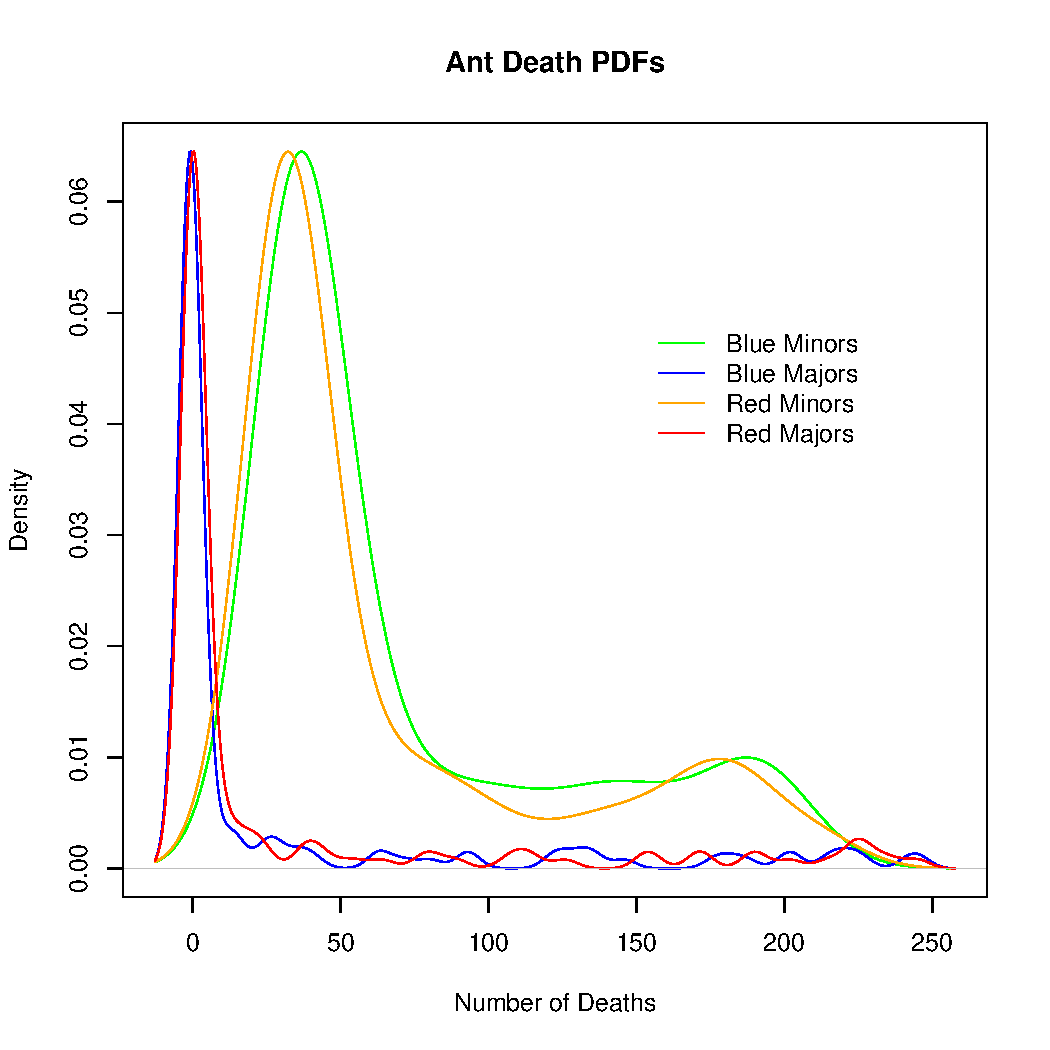
\includegraphics[scale=0.80]{partb1v1.pdf}
\caption{Probability density function for $f = 0.25, p = 0.5$}
\label{partb1fig}
\end{figure}

\begin{figure}[h!]
\centering
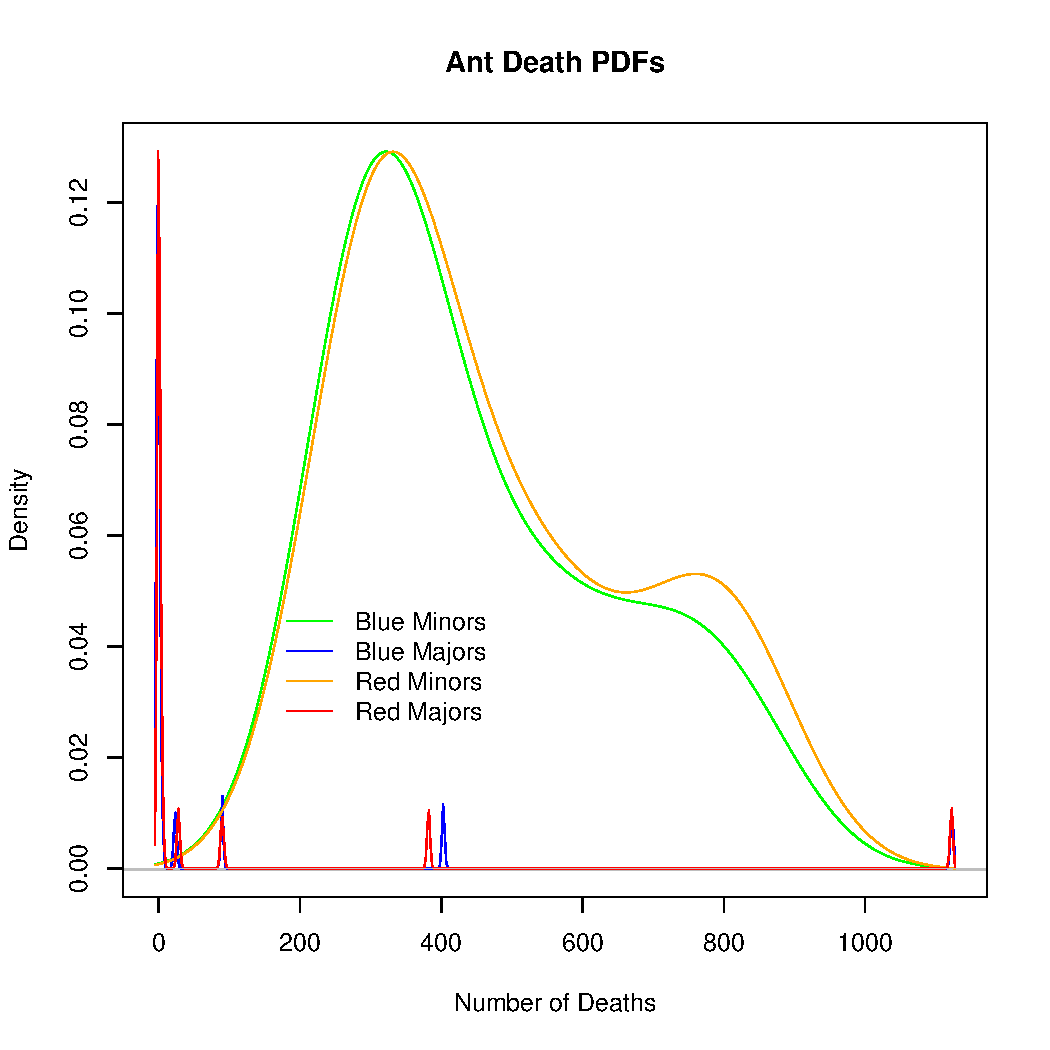
\includegraphics[scale=0.80]{partb2v1.pdf}
\caption{Probability density function for $f = 0.12, p = 0.04$}
\label{partb2fig}
\end{figure}

\begin{figure}[h!]
\centering
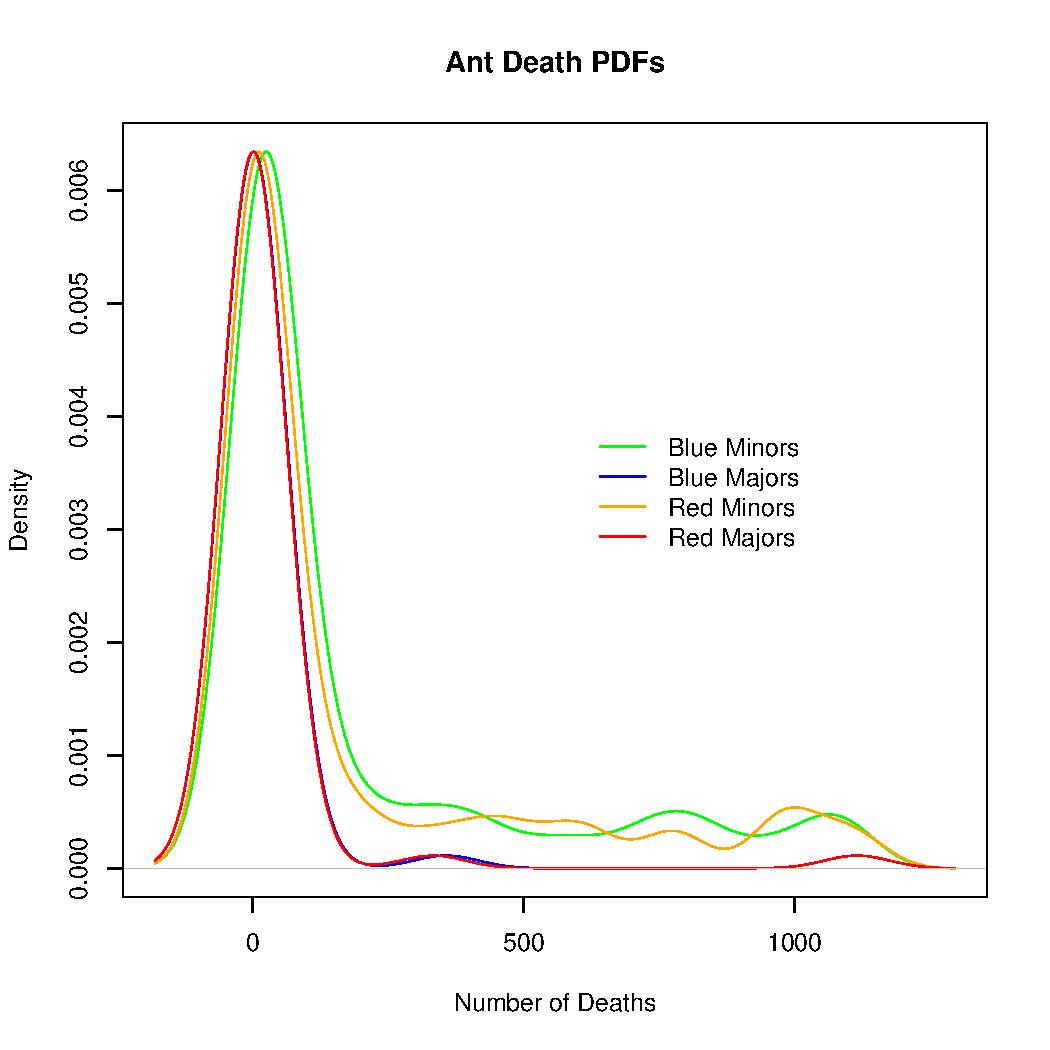
\includegraphics[scale=0.80]{partb3v1.pdf}
\caption{Probability density function for $f = 0.04, p = 0.21$}
\label{partb3fig}
\end{figure}

\item (0.5, 0.25): Qualitatively, this doesn't appear to allow for either side to be 
particularly effective.  The majors tend to just stick around, while the 
smaller numbers of minors means both less minor deaths (pred), and less major 
deaths (pred), with neither tribe controlling the entire grid.

(0.04, 0.12): This chart is startlingly different.  Most obviously, the number 
of major deaths that occur are very small, which is due to the small 
probability that a major ant gets born each step.  In addition, this allows the 
minor ants to form the vast majority of the battlefronts that appear on the 
grid.  While the simulation runs, the minor ants appear to steadly hold the 
battlelines in place.  The battlefronts mainly shift only when a major ant ends 
up at the edge of tribe's region, when it is possible for the major ant to 
break through the boundaries of the other tribe's region.

(0.21, 0.04): Different again.  In this case, there are very well defined 
regions of red and blue ants, similar to the 0.04, 0.12 case.  In this 
situation, there tend to be fewer different regions and as a result each 
red/blue region is larger.  Again, the minor ants appear to form stable edges 
to each region, while major ants born either in the empty lines or the edges of 
the coloured regions push the battlefronts into new territory.  A further 
effect of the larger territories occupied by each tribe is that the overall 
death counts for both major and minor ants are low and similar.  This is 
because most of the ants from each tribe aren't located at the edge of a tribal 
region, so they have no opportunity to get involved in battles with enemy ants.

\item Having different f values for 
\end{enumerate}
hasdlfkjasd
